\documentclass[a4paper,14pt]{extarticle}
\usepackage{geometry}
\usepackage[T1]{fontenc}
\usepackage[utf8]{inputenc}
\usepackage[english,russian]{babel}
\usepackage{amsmath}
\usepackage{amsthm}
\usepackage{amssymb}
\usepackage{fancyhdr}
\usepackage{setspace}
\usepackage{graphicx}
\usepackage{colortbl}
\usepackage{tikz}
\usepackage{pgf}
\usepackage{subcaption}
\usepackage{listings}
\usepackage[colorlinks, linkcolor=blue, urlcolor=blue]{hyperref}
\usepackage{indentfirst}
\graphicspath{{images/}}%путь к рисункам
\usepackage{mathptmx}

\makeatletter
\renewcommand{\@biblabel}[1]{#1.} % Заменяем библиографию с квадратных скобок на точку:
\makeatother

\geometry{left=2.5cm}% левое поле
\geometry{right=1.5cm}% правое поле
\geometry{top=1.5cm}% верхнее поле
\geometry{bottom=1.5cm}% нижнее поле
\renewcommand{\baselinestretch}{1.5} % междустрочный интервал

\newcommand{\bibref}[3]{\hyperlink{#1}{#2 (#3)}} % biblabel, authors, year

\renewcommand{\theenumi}{\arabic{enumi}}% Меняем везде перечисления на цифра.цифра
\renewcommand{\labelenumi}{\arabic{enumi}}% Меняем везде перечисления на цифра.цифра
\renewcommand{\theenumii}{.\arabic{enumii}}% Меняем везде перечисления на цифра.цифра
\renewcommand{\labelenumii}{\arabic{enumi}.\arabic{enumii}.}% Меняем везде перечисления на цифра.цифра
\renewcommand{\theenumiii}{.\arabic{enumiii}}% Меняем везде перечисления на цифра.цифра
\renewcommand{\labelenumiii}{\arabic{enumi}.\arabic{enumii}.\arabic{enumiii}.}% Меняем везде перечисления на цифра.цифра


\begin{document}
    \begin{titlepage}
    \newpage

    {\setstretch{1.0}
    \begin{center}
        Федеральное государственное автономное образовательное учреждение высшего образования «Национальный исследовательский университет «Высшая школа экономики»
        \\
        \bigskip
        Факультет компьютерных наук \\
        Основная образовательная программа \\
        Прикладная математика и информатика \\
    \end{center}
    }

    \vspace{8em}

    \begin{center}
    {\Large ГРУППОВАЯ КУРСОВАЯ РАБОТА}
        \\
        \textsc{\textbf{
        Программный проект на тему
        \linebreak
        "Решения на основе компьютерного зрения для проектов в городской среде"}}
    \end{center}

    \vspace{2em}

    {\setstretch{1.0}
    \hfill\parbox{16cm}{
    \hspace*{5cm}\hspace*{-5cm}Выполнили студент группы 171, 3 курса,\\
    Биршерт Алексей Дмитриевич,\\
    Шабалин Александр Михайлович\\

    \hspace*{5cm}\hspace*{-5cm}Руководитель КР:\\
    старший преподаватель Соколов Евгений Андреевич
    \\

    %\hspace*{5cm}\hspace*{-5cm}Куратор:\hfill < степень>, <звание>, <ФИО полностью>\\

    \hspace*{5cm}\hspace*{-5cm}Консультант:\\
    научный сотрудник Лобачева Екатерина Максимовна\\
    }
    }

    \vspace{\fill}

    \begin{center}
        Москва 2020
    \end{center}

\end{titlepage}
    \newpage

    {
    \hypersetup{linkcolor=black}
    \tableofcontents
    }

    \newpage

    \begin{abstract}
        При проведении антропологических исследований часто необходимо обработать данные внушительных объемов.
        Существует вариант обработать все эти данные вручную, однако такой метод слишком затратен по времени и трудовым ресурсам.
        В нашей проектной работе мы решаем задачу автоматизации обработки изображений.
        Наша задача заключается в классификации гендерных и возрастных групп людей, запечатленных на фотографии.
        В процессе решения возникли несколько подзадач.
        Первая - выделение лица на изображении.
        Решение этой задачи позволяет сконцентрироваться на самых важных для нас признаках.
        Вторая - проверка того, что выделенное на снимке лицо принадлежит живому человеку, а не напечатано на рекламном щите или является скульптурой.
        Решение этой задачи позволяет уменьшить шум в данных и повысить точность статистик возрастных и гендерных групп, вычисляемых по фотографиям.
        В своём решении мы комбинируем различные известные подходы для достижения наилучшего результата.
        \\
        \small \textbf{\textit{Ключевые слова---}}Определение возраста и пола, Распознавание лиц, Компьютерное зрение, Глубокое обучение, Антропология \\

        When conducting anthropological studies, it is often necessary to process a large amount of data.
        There is an option to process all this data manually, but this method is too time-consuming and labor-intensive.
        In our work, we solve the problem of automating image processing.
        Our task is to classify the gender and age groups of people captured in the photograph.
        In the process of solving several subtasks arose.
        The first is the selection of the face in the image.
        The solution to this problem allows us to concentrate on the most important features.
        The second is to verify that the face highlighted in the picture belongs to a living person, and is not printed on a billboard or is a sculpture.
        The solution to this problem allows us to reduce noise in the data and improve the accuracy of statistics of age and gender groups calculated from photographs.
        In our decision, we combine various well-known approaches to achieve the best result.
        \\
        \small \textbf{\textit{Keywords---}}Age and gender classification, Facial recognition, Computer vision, Deep learning, Anthropology
        \\
        \newpage
    \end{abstract}


    \section{Введение}\label{sec:введение}

    На сегодняшний день человечество владеет огромными объемами данных, и во многих сферах деятельности приходится каким-либо образом с ними взаимодействовать.
    Одной из таких сфер является антропология.
    Для изучения человеческого развития и культуры необходимо наблюдать за человеком и анализировать его поступки и предпочтения.
    Одной из задач антропологов является облагораживание города.
    Для ее выполнения им нужно знать, где горожанам не хватает детской площадки или парка, где требуется произвести ремонт или реконструкцию здания.
    Хорошим источником информации о людях являются фотографии жителей какого-либо населенного пункта, ведь из них можно узнать, какие достопримечательности или объекты архитектуры наиболее привлекают людей, к каким возрастным и гендерным группам относятся эти люди.
    Никто не хочет тратить свое время и силы на просмотр тысяч фотографий и выделение из них полезных данных, когда гораздо удобнее и выгоднее автоматизировать этот рутинный процесс там, где это возможно.
    \par Все известные подходы к классификации возрастных групп людей по фотографии заключаются в анализе изображения лица.
    Самые ранние (\cite{age1994}) основывались на различиях в пропорциях и размерах черт лица в зависимости от возраста - так называемые антропометрические модели (\cite{unfiltered}).
    Все они вычисляли координаты точек на лице и в дальнейшем их анализировали.
    Более поздние методы (\cite{hassner}) опирались на использование сверточных нейронных сетей различной глубины или полнокомпонентных сверточных нейронных сетей (\cite{INDIA}).
    \par Первые подходы к классификации пола использовали фотографии лица низкого разрешения - до 20 на 20 пикселей, и обучали на них различные типы классификаторов (\cite{smoll}).
    Позднее стали использовать LBP для выявления новых признаков (\cite{lbp_age}), использовать сверточные нейронные сети (\cite{hassner,INDIA}).
    \par В ходе выполнения работы мы не будем предлагать каких-либо новых методов, однако мы используем ряд различных уже существующих технологий машинного обучения, которые могут быть применимы в решении самых разных задач.
    В итоге мы получим алгоритм, способный перебирать большие объемы фотографий, находить на них нужные объекты и собирать важные статистики для помощи в проведении исследований.
    \par Дальнейшая работа описана в следующих главах - обзор литературы, распознавание лиц, отличие "живого" \, лица от напечатанного, классификация лиц людей и скульптур, классификация гендерных и возрастных групп.
    Отличие "живого" \, лица от напечатанного выполнено Александром Шабалиным, классификация лиц людей и скульптур Алексеем Биршертом.
    \newpage


    \section{Обзор литературы}\label{sec:обзор-литературы}

    \subsection{Классификация возраста и пола}\label{subsec:классификация-возраста-и-пола}
    \par Задачи определения пола и возраста человека находят применение в разных сферах жизни человека, в наружном наблюдении, в антропологии, в биометрической идентификации.
    Современные подходы к этой задаче опираются на сверточные нейронные сети.
    Так, например, в статье~\cite{hassner} описано решение с помощью сверточной сети небольшой глубины.
    Для классификации возраста и пола используется одна и та же архитектура.
    Нейронная сеть состоит из трёх свёрточных слоёв и двух полносвязных, небольшой размер сети объясняется желанием быть физичным в распознавании лиц и нежеланием переобучиться.
    Точность по классификации пола была 86.8 $\pm$ 1.4\%, возрастных групп - 50.7 $\pm$ 5.1\% для точного попадания в группу и 84.7 $\pm$ 2.2\% для попадания в правильную или соседнюю.
    \par В статье~\cite{INDIA} описан алгоритм анализа лица с помощью пяти сверточных нейросетей, получающих изображения лица целиком, левого и правого глаза, носа и рта соответственно.
    Итоговое решение принимается на основе выходов всех пяти нейросетей.
    Нейросеть, получающая на вход всё изображение лица, имеет три сверточных слоя, прочие по два.
    Точность по классификации пола достигла 89.6 $\pm$ 1.3\%, возрастных групп - 54.3 $\pm$ 3.5\% для точного попадания в группу и 87.6 $\pm$ 1.9\% для попадания в правильную или соседнюю, что является значительным улучшением результата предыдущей статьи.
    \newpage


    \section{Детектирование лица}\label{sec:детектирование-лица}
    ЧТОТО СДЕЛАЛИ ДА
    \newpage


    \section{Классификация гендерных и возрастных групп}\label{sec:классификация-гендерных-и-возрастных-групп}
    Эта часть выполнена Алексеем Биршертом. \\

\subsection{Описание выбранного метода}\label{subsec:описание-метода}
Для предсказания пола и возраста используются две нейронные сети, состоящие из основной и выходной моделей каждая.
В качестве основной модели используется глубокая нейронная сеть ResNet-18, без последнего полносвязного слоя.
В качестве выходной модели используется персептрон из двух полносвязных слоёв с нелинейностью ReLU и дропаутом между ними.
На вход основной модели подаются изображения 227 на 227 пикселей, 3 канала цвета - R, G, B,
выход основной модели подаётся на вход выходной модели.
Выходом нейросети будет выход выходной модели.
Первая нейронная сеть предназначена для классификации пола и имеет в выходной модели 512 и 256 входных и выходных нейронов в первом слое, 256 и 2 во втором соответственно.
Вторая нейронная сеть предназначена для классификации возраста и имеет в выходной модели 512 и 512 входных и выходных нейронов в первом слое, 512 и 101 во втором соответственно.
На вход подаются фотографии лиц людей, выделенные и выровненные с помощью модели детектирования лиц.
Предсказанный пол определяется как номер выходного нейрона соответствующей нейронной сети с максимальным значением -
первый это "женский"\,, второй "мужской".
Предсказанный возраст определяется следующим образом: сначала для вектора значений выходных нейронов
соответсвующей нейронной сети применяется преобразование софтмакс, затем значения умножаются на соответствующий
им возраст.
После вектор суммируется - получаем матожидание возраста при вероятностном распределении, выданном моделью.
\[AGE = \sum\limits_{i = 0}^{100}i \cdot softmax(x)_i, \quad softmax(x)_i = \frac{\exp(x_i)}{\sum\limits_{j =
0}^{100}\exp(x_j)}.\]

\subsection{Описание и подготовка данных}\label{subsec:описание-данных}
В качестве датасета для обучения двух вышеописанных моделей были избраны датасеты IMDB-WIKI-101~\cite{imdb_db} и FGNET~\cite{fgnet}.
Оба датасета имеют в мета-данных метки пола "женщина" или "мужчина"\, и имеют метки возраста в виде целых чисел от 0 до 100 включительно.
Распределение возраста в датасете IMDB-WIKI-101 имеет вид нормальной кривой со средним около 35 лет,
имея малое количество объектов с возрастом меньше 10 лет или больше 90.
Для увеличения количества данных с возрастом до 10 лет был избран датасет FGNET, в котором большая часть объектов это дети до 15 лет.
Для улучшения сходимости нейронных сетей была произведена предобработка всех объектов -
в итоговую выборку не были включены следующие объекты:
объекты с плохо различимыми лицами (показатель уверенности модели распознавания лиц в том, что это лицо, ниже фиксированного значения),
объекты с некорректно заполненными данными по полу/возрасту,
объекты со слишком маленькими фотографиями.
На каждом изображении было выделено и выровнено лицо.
Отступ от границы лица был поставлен на 40\%, чтобы лицо целиком оказывалось на выделенной зоне.
Итого было получено около 200 тысяч объектов, которые были в дальнейшем поделены
с сохранением баланса классов 1 к 19 на валидационную и обучающую выборки соответственно.
\par В качестве датасета для тестирования был избран датасет Adience~\cite{adience}, по которому известно большое количество результатов различных моделей.
Из него были исключены объекты с некорректным описанием пола или возраста.
Итого было получено почти 11 тысяч объектов для тестовой выборки.
В Adience метки возраста в формате 8 групп - 0: [0, 2], 1: [4, 6], 2: [8, 12], 3: [15, 20], 4: [25, 32], 5: [38, 43], 6: [48, 53], 7: [60, 100].
В связи с этим, необходимо было решить как относить к этим группам метки реального возраста от 0 до 100.
Было принято решение относить к той группе, граница которой ближе по модулю, в случае равенства относить к первой в порядке следования.

\subsection{Постановка задач обучения}\label{subsec:постановка-задач-обучения}
Задача классификации пола является задачей бинарной классификации, целевая переменная для одного объекта это число 0 или 1.
Для обучения была выбрана перекрестная энтропия - функция ошибки со следующей формулой:
\[loss(x, y) = -x_y + \log\left(\sum\limits_{j=1}^{K}\exp(x_j)\right),\] где $x$ - вектор значений выходных нейронов нейронной сети,
$y$ - целевая переменная.
Для оценки качества классификации использовались метрика доля правильных ответов, так как выборки сбалансированны по полу.
\par Задача классификации возраста является задачей многоклассовой классификации.
Если смотреть на задачу предсказания возраста по фотографии с точки зрения человека,
человек гораздо точнее способен угадать диапазон возраста, нежели точный возраст.
Поэтому задача классификации возраста была интерпретирована как задача с множественными правильными ответами -
каждому объекту может соответствовать набор правильных классов.
Целевой переменной для одного объекта служил вектор из нулей и единиц, единицы на позициях правильных классов.
Правильные классы определялись как значения возраста, которые отличаются по модулю от правильного не больше,
чем на фиксированное число, которое было гиперпараметром (далее об этом в разделе эксперименты~\ref{subsec:эксперименты}).
Для обучения была выбрана бинарная перекрестная энтропия -
\[loss(x, y) = sum(L), \quad L = \{l_1, \dots l_N\}, \quad l_i = \left(y_i \log(x_i) + (1 - y_i) \log(1 - x_i)\right),\]
где $x$ это вектор значений выходных нейронов нейронной сети после применения сигмоидного преобразования,
$y$ - целевая переменная.
Для оценки качества классификации использовались средний модуль отклонения (далее MAE)
и доля объектов, у которых MAE не превышает фиксированного числа (далее CS-5).

\subsection{Эксперименты}\label{subsec:эксперименты}
В качестве основных было рассмотрено два варианта - нейронная сеть на основе статьи~\cite{ror} и нейронная сеть на основе статьи~\cite{lstm}.
Однако стоит заметить, что анализ и использование модели из второй статьи на порядок сложнее, так как помимо сверточных нейронных сетей там используется блок LSTM,
для работы с которым необходимо иметь соответствующий опыт.
Поэтому было принято решение базировать работу на основе первой статьи, слегка упростив архитектуру.
\par Необходимо было решить вопрос выбора архитектуры базовой модели.
Всего было опробовано три различных архитектуры - MobileNet, ShuffleNet~\cite{shuffle}, ResNet.
Лучше всего себя проявила архитектура ResNet-18.
MobileNet и ShuffleNet незначительно быстрее, не смотря на реализацию, однако достаточно сильно проигрывали в качестве.
В итоге была выбрана архитектура ResNet.
\par Так как ResNet-18 предобучен на датасете ImageNet-1000, он имеет очень хорошую способность выделять признаки из изображения.
Известно, что первые (входные) сверточные слои обученных моделей очень похожи между собой даже для различных задач.
Таким образом, было решено веса первого сверточного слоя ResNet-18 взять из предобученной на ImageNet-1000 модели и заморозить в процессе обучения,
дообучая веса всех остальных слоев.
\par Вторым необходимо было решить вопрос выбора количества моделей - одна нейронная сеть из общей базовой модели и двух паралелльных выходных моделей
или две отдельные нейронные сети из основной и выходной модели.
Однако стоит заметить, что для обеих задач нейронная сеть и должна выделять признаки лица, признаки,
отвечающие за пол, несколько отличаются от признаков, которые соответствуют возрасту.
Также в силу использования функций ошибки,
которые имеют разный масштаб и решают частично разные задачи на моменте основной модели,
и сложности в подборе гиперпараметров для комбинирования этих функций ошибки,
нейронная сеть из одной общей основной модели очень плохо сходилась и достигала намного меньшего качества во всех проведенных экспериментах.
В итоге было принято решение использовать две паралелльные нейронные сети, по одной на решаемую задачу.
\par В процессе подбора гиперпараметров для обучения были выбраны следующие значения: темп обучения был выставлен на $1e-3$ для первых 40 эпох,
далее $1e-4$ для модели предсказания возраста, $1e-4$ для первых 30 эпох и $2e-5$ далее для модели предсказания пола;
коэффициент $L2$ регуляризации был установлен на $1e-3$ для обеих моделей;
размер батча был установлен в силу ограничений на память ГПУ и в качестве дополнительной регуляризации при обучении на 128;
размер входных картинок 227 на 227 пикселей;
дропаут 0.1 перед 4 слоём ResNet, 0.2 перед первым полносвязным слоём и 0.4 между слоями.
В качестве размера окна для правильного возраста после сравнений было выбрано число в 5 лет.
Модели, обученные с такими гиперпараметрами показали наилучшие результаты.
\par В процессе выбора аугментации были выбраны следующие трансформации -
в процессе обучения при проходе по датасету каждое изображение преобразовывалось к квадрату 256 на 256 пикселей,
затем из него выбирался случайный квадрат со стороной 227 пикселей,
который с вероятностью $1/2$ мог быть отражен вдоль вертикальной оси, проходящей через его центр.
Во время тестирования каждое изображение преобразовывалось к квадрату 256 на 256 пикселей,
затем из него по центру вырезался квадрат со стороной 227 пикселей.

\subsection{Результаты}\label{subsec:результаты}
Как итог модели показали следующие показатели метрик на обучающей и валидационной выборках: для возраста MAE 5 и 5.6 соответственно,
CS-5 0.71 и 0.69 соответственно, для пола Accuracy 0.94 и 0.93 соответственно.
\par Модель показала следующие результаты на датасете Adience: для возраста Exact-accuracy $49.1\% \pm 4.1 \%$ и One-off-accuracy $84.4\% \pm 3.6 \%$,
для пола значение метрики Accuracy $83.7\% \pm 2.7\%$.
Значения метрик получаются подсчетом соответствующих метрик для каждой из 8 возрастных групп
и вычисления среднего арифметического от посчитанных показателей.
\par Всего было написано более 2300 строк кода на языке программирования Python3,
все модели были написаны и обучены с использованием фреймворка машинного обучения PyTorch.
\newpage

\subsection{Примеры работы модели}\label{subsec:примеры-работы-модели2}
\begin{figure}[h]
    \center
    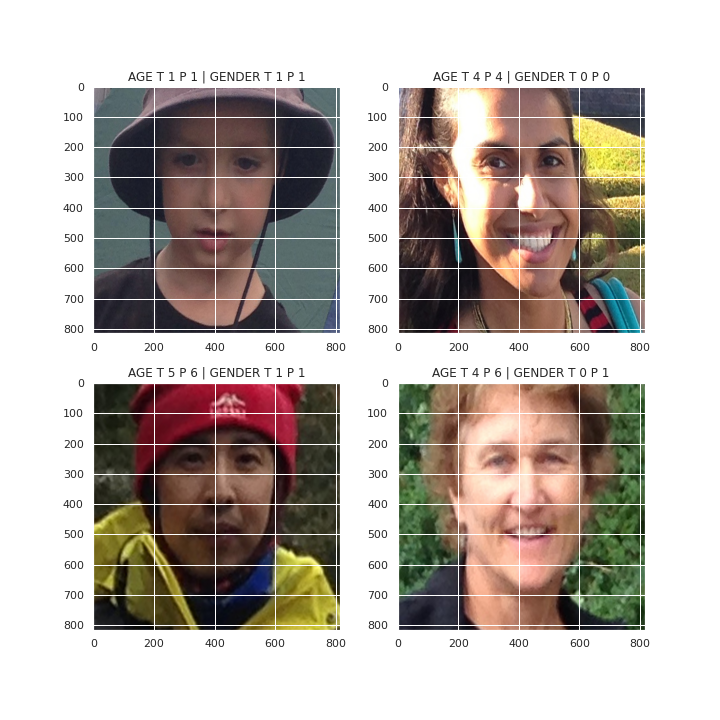
\includegraphics[width=0.9\linewidth]{images/image.png}
    \caption{Пример работы модели на 4 случайных лицах из датасета Adience}
    \label{ris:images/image.png}
\end{figure}
Здесь мы видим примеры ответов модели на случайных изображениях из датасета Adience.
Для каждого изображения написана информация про правильный ответ и ответ модели по следующему формату -
сначала идёт название целевой переменной, потом правильный ответ после метки \textbf{T}, потом ответ модели после метки \textbf{P}.
Напомним, что метки пола имеют соответствие 0 - "женщина"\,, 1 - "мужчина"\,.
Метки возраста - 0: [0, 2], 1: [4, 6], 2: [8, 12], 3: [15, 20], 4: [25, 32], 5: [38, 43], 6: [48, 53], 7: [60, 100].


    \section{Список литературы}\label{sec:список-литературы}
    \begin{thebibliography}{0}
    \bibitem{age1994}\hypertarget{age1994}{}
    \href{https://pdfs.semanticscholar.org/20cb/d360c8e6f70aac3e11853d81e3b18e4866c2.pdf}
    {Age Classification from Facial Images.
    Young H. Kwon, Niels da Vitoria Lobo.
    In IEEE 1994}

    \bibitem{unfiltered}\hypertarget{unfiltered}{}
    \href{https://www.openu.ac.il/home/hassner/Adience/EidingerEnbarHassner_tifs.pdf}
    {Age and Gender Estimation of Unfiltered Faces.
    Eran Eidinger, Roee Enbar, Tal Hassner.
    In IEEE 2014}

    \bibitem{hassner}\hypertarget{hassner}{}
    \href{https://talhassner.github.io/home/projects/cnn_agegender/CVPR2015_CNN_AgeGenderEstimation.pdf}
    {Age and Gender Classification using Convolutional Neural Networks.
    Gil Levi, Tal Hassner.
    In IEEE 2015}

    \bibitem{INDIA}\hypertarget{INDIA}{}
    \href{https://ieeexplore.ieee.org/document/8282221}
    {Age/gender classification with whole-component convolutional neural networks (WC-CNN).
    Chun-Ting Huang, Yueru Chen, Ruiyuan Lin, C.-C. Jay Kuo.
    In IEEE 2018}

    \bibitem{smoll}\hypertarget{smoll}{}
    \href{https://merl.com/publications/docs/TR2002-12.pdf}
    {Learning Gender with Support Faces.
    Baback Moghaddam, Ming-Hsuan Yang.
    In IEEE 2002}

    \bibitem{lbp_age}\hypertarget{lbp_age}{}
    \href{https://link.springer.com/chapter/10.1007/978-3-540-74549-5_49}
    {Demographic Classification with Local Binary Patterns.
    Zhiguang Yang, Haizhou Ai. In ICB 2007}

    \bibitem{face_detection}\hypertarget{face_detection}{}
    \href{http://www.face-rec.org/algorithms/Boosting-Ensemble/16981346.pdf}
    {Robust Real-Time Face Detection.
    Paul Viola, Michael J. Jones.
    In IEEE 2003}

    \bibitem{face_detection2}\hypertarget{face_detection2}{}
    \href{http://rodrigob.github.io/documents/2014_eccv_face_detection_with_supplementary_material.pdf}
    {Face detection without bells and whistles.
    Makrus Mathias, Rodrigo Beneson, Marco Pedersoli, Lus Van Gool.
    In ECCV 2014}

    \bibitem{face_detection3}\hypertarget{face_detection3}{}
    \href{https://arxiv.org/abs/1905.01585}
    {Accurate Face Detection for High Performance.
    Faen Zhang, Xinyu Fan, Guo Ai, Jianfei Song, Yongqiang Qin, Jiahong Wu. In ArXiv 2019}

    \bibitem{resnet}\hypertarget{resnet}{}
    \href{https://arxiv.org/abs/1512.03385}
    {Deep Residual Learning for Image Recognition.
    Kaiming He, Xiangyu Zhang, Shaoqing Ren, Jian Sun.
    In IEEE 2015}

    \bibitem{align}\hypertarget{align}{}
    \href{http://www.csc.kth.se/~vahidk/papers/KazemiCVPR14.pdf}
    {One Millisecond Face Alignment with an Ensemble of Regression Trees.
    Vahid Kazemi and Josephine Sullivan.
    In IEEE 2014}

    \bibitem{lbp}\hypertarget{lpb}{}
    \href{https://arxiv.org/abs/1511.06316}
    {Face Anti-Spoofing Based on Color Texture Analysis.
    Zinelabidine Boulkenafet, Jukka Komulainen, Abdenour Hadid.
    In IEEE 2015}

    \bibitem{lbp2}\hypertarget{lpb2}{}
    \href{https://arxiv.org/abs/1803.11097}
    {Learning Deep Models for Face Anti-Spoofing: Binary or Auxiliary Supervision.
    Yaojie Liu, Amin Jourabloo, Xiaoming Liu.
    In IEEE/CVF 2018}

    \bibitem{lbp3}\hypertarget{lpb3}{}
    \href{https://arxiv.org/abs/1904.02860}
    {Deep Tree Learning for Zero-shot Face Anti-Spoofing.
    Yaojie Liu, Joel Stehouwer, Amin Jourabloo, Xiaoming Liu.
    In IEEE/CVF 2019}

    \bibitem{pfid}\hypertarget{pfid}{}
    \href{https://arxiv.org/abs/1907.02642}
    {Primate Face Identification in the Wild.
    Ankita Shukla, Gullal Singh Cheema, Saket Anand, Qamar Qureshi, Yadvendradev Jhala.
    In PRICAI 2019}

    \bibitem{pfid2}\hypertarget{pfid2}{}
    \href{https://arxiv.org/abs/1406.4773}
    {Deep Learning Face Representation by Joint Identification-Verification.
    Yi Sun, Xiaogang Wang, Xiaoou Tang.
    In NIPS 2014}

    \bibitem{pfid3}\hypertarget{pfid3}{}
    \href{https://ydwen.github.io/papers/WenECCV16.pdf}
    {A Discriminative Feature Learning Approach for Deep Face Recognition.
    Yandong Wen, Kaipeng Zhang, Zhifeng Li, and Yu Qiao.
    In ECCV 2016}

    \bibitem{densenet}\hypertarget{densenet}{}
    \href{https://arxiv.org/abs/1608.06993}
    {Densely Connected Convolutional Networks.
    Gao Huang, Zhuang Liu, Laurens van der Maaten, Kilian Q. Weinberger.
    In IEEE 2016}

    \bibitem{NUAA}\hypertarget{NUAA}{}
    \href{http://parnec.nuaa.edu.cn/xtan/data/nuaaimposterdb.html}
    {NUAA Photograph Imposter Database}

    \bibitem{lfw}\hypertarget{lfw}{}
    \href{http://vis-www.cs.umass.edu/lfw/}
    {Labeled Faces in the Wild Database}

    \bibitem{IMDB-WIKI}\hypertarget{IMDB-WIKI}{}
    \href{https://data.vision.ee.ethz.ch/cvl/rrothe/imdb-wiki/}
    {IMDB-WIKI Database}

    \bibitem{bug}\hypertarget{bug}{}
    \href{https://ibug.doc.ic.ac.uk/resources/300-W/}
    {300 Faces In-the-Wild Database}

\end{thebibliography}

\end{document}